\documentclass[10pt]{beamer}

\mode<presentation>{% Settings
    % link to view http://www.hartwork.org/beamer-theme-matrix/
    % ------------------------------------------------------------------------------
    % Slide Themes
    % ------------------------------------------------------------------------------
    %\usetheme{default}
    %\usetheme{AnnArbor}
    %\usetheme{Antibes}
    %\usetheme{Bergen}
    \usetheme{Berkeley}
    %\usetheme{Berlin}
    %\usetheme{Boadilla}
    %\usetheme{CambridgeUS}
    %\usetheme{Copenhagen}
    %\usetheme{Darmstadt}
    %\usetheme{Dresden}
    %\usetheme{Frankfurt}
    %\usetheme{Goettingen}
    %\usetheme{Hannover}
    %\usetheme{Ilmenau}
    %\usetheme{JuanLesPins} % rounded title, gradient at top with section, no bottom bar
    %\usetheme{Luebeck}     % square title, toc at top of each slide
    %\usetheme{Madrid}      % rounded title
    %\usetheme{Malmoe}
    %\usetheme{Marburg}
    %\usetheme{Montpellier}
    %\usetheme{PaloAlto}
    %\usetheme{Pittsburgh}
    %\usetheme{Rochester}
    %\usetheme{Singapore}
    %\usetheme{Szeged}
    %\usetheme{Warsaw}

    % ------------------------------------------------------------------------------
    % Color Schemes
    % ------------------------------------------------------------------------------
    %\usecolortheme{default}
    %\usecolortheme{albatross}  % blue background with darker blue
    %\usecolortheme{beaver}     % gray with red
    %\usecolortheme{beetle}     % gray background
    %\usecolortheme{crane}      % orange
    \usecolortheme{dolphin}     % white with purple
    %\usecolortheme{dove}       % all white
    %\usecolortheme{fly}        % all gray including background
    %\usecolortheme{lily}       % white with blue
    %\usecolortheme{orchid}     % default blue
    %\usecolortheme{rose}       % default blue
    %\usecolortheme{seagull}    % darker gray than seahorse
    %\usecolortheme{seahorse}   % light gray blueish tint
    %\usecolortheme{whale}      % default blue
    %\usecolortheme{wolverine}  % yellow with a little blue

    %\setbeamertemplate{footline} % To remove the footer line in all slides uncomment this line
    %\setbeamertemplate{footline}[page number] % To replace the footer line in all slides with a simple slide count uncomment this line
    \setbeamertemplate{navigation symbols}{} % To remove the navigation symbols from the bottom of all slides uncomment this line
    \setbeamertemplate{bibliography item}{\insertbiblabel} % to number bibliography entries
}

\usepackage{Logemann}
\usepackage{Integral}
\usepackage{LinearAlgebra}
\usepackage{Derivative}
\usepackage{Vector}
\usepackage{Sum}
\usepackage{SetTheory}
\usepackage{booktabs}
\usepackage[backend=biber]{biblatex}
\addbibresource{refs.bib}

\title[]{Discontinuous Galerkin Method for Solving Thin Film Equations} % The short title
% appears at the bottom of every slide, the full title is only on the title page

\author{Caleb Logemann \and James Rossmanith} % Your name
\institute[Iowa State University]{% Your institution as it will appear on the bottom of every slide, may be shorthand to save space
Mathematics Department,\\ Iowa State University \\ % Your institution for the title page 
\medskip
\textit{logemann@iastate.edu}} % Your email address

\date{May 13, 2019} % Date, can be changed to a custom date

\begin{document}
  \begin{frame}
    \titlepage{}
  \end{frame}

  \begin{frame}
    \frametitle{Overview}
    \tableofcontents
  \end{frame}

  \section{Introduction}
    \begin{frame}
      \frametitle{Motivation}
      \begin{itemize}
        \item Aircraft Icing
        \item Runback
      \end{itemize}
      \begin{center}
        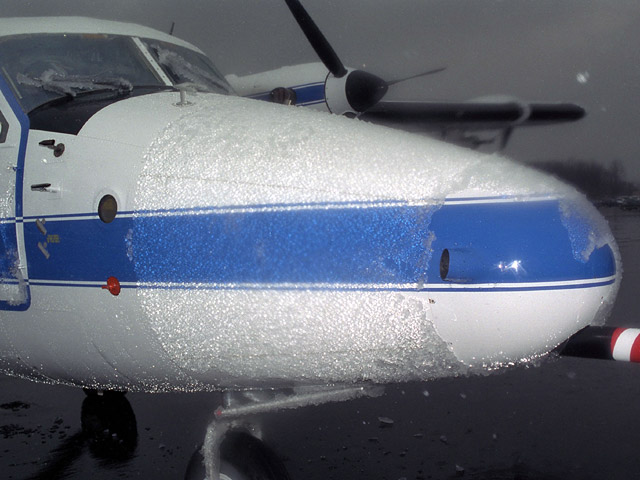
\includegraphics[scale=0.2]{Figures/Icing_on_a_plane.jpg}
        \hspace{0.1in}
        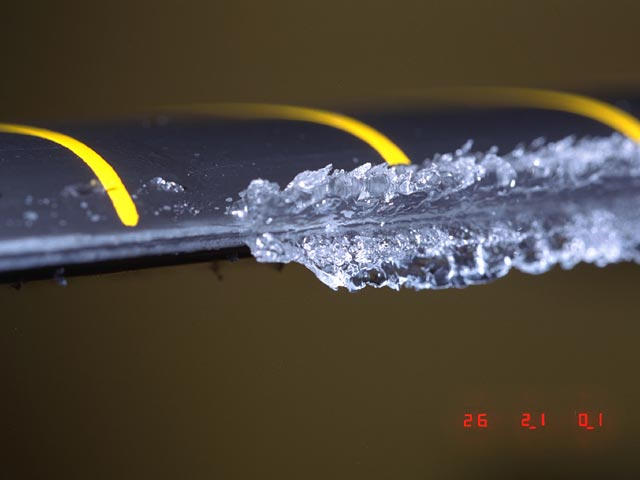
\includegraphics[scale=0.2]{Figures/Icing_on_a_rotor.jpg}
      \end{center}
      \begin{itemize}
        \item Industrial Coating
      \end{itemize}
    \end{frame}

  \section{Derivation}
    \begin{frame}
      \frametitle{Model Equations}
      \begin{center}
        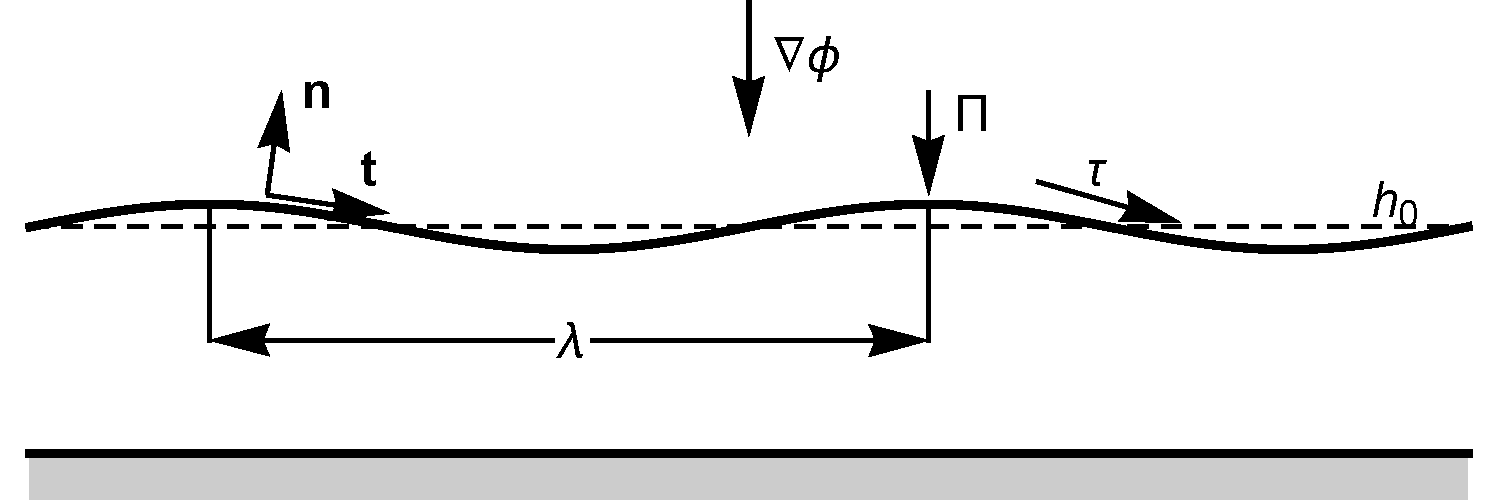
\includegraphics[scale=0.35]{Figures/ThinFilm.pdf}
      \end{center}
      \begin{itemize}
        \item Incompressible Navier-Stokes Equation
          \begin{align*}
            u_x + w_z &= 0 \\
            \rho\p{u_t + u u_x + w u_z} &= -p_x + \mu \Delta u - \phi_x \\
            \rho\p{w_t + u w_x + w w_z} &= -p_z + \mu \Delta w - \phi_z \\
            w &= 0, u = 0 &\text{at } z = 0 \\
            w &= h_t + u h_x &\text{at } z = h\\
            \v{T} \cdot \v{n} &= \p{-\kappa \sigma + \Pi}\v{n} + \p{\pd{\sigma}{s} + \tau}\v{t} &\text{at } z = h
          \end{align*}
      \end{itemize}
    \end{frame}

    \begin{frame}
      \frametitle{Nondimensionalization}
      \begin{center}
        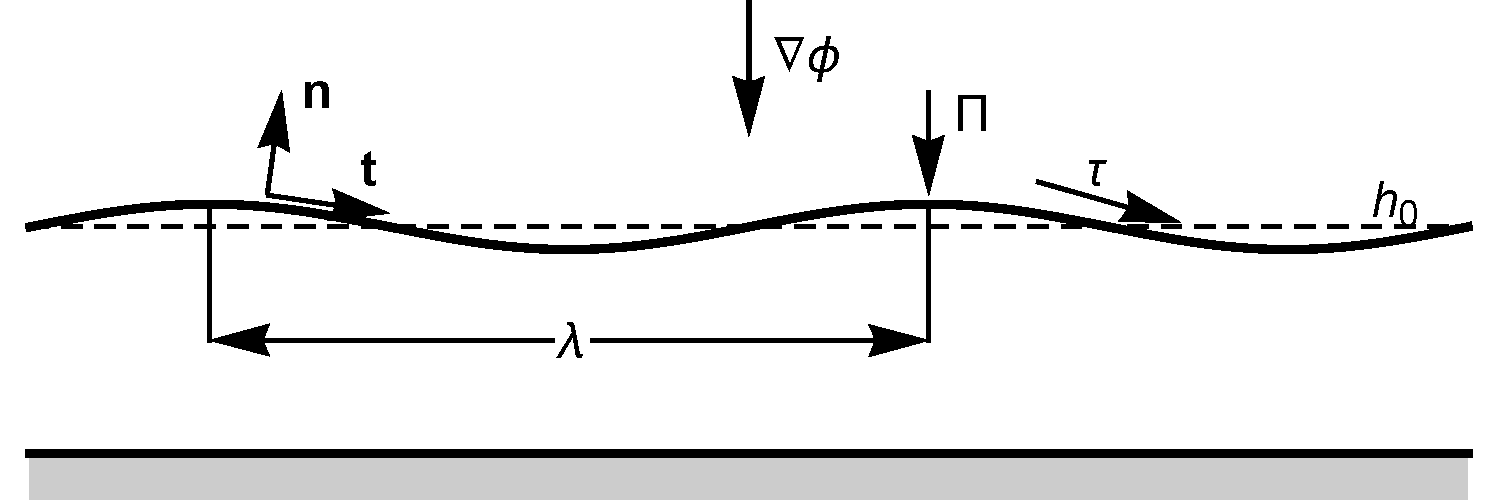
\includegraphics[scale=0.35]{Figures/ThinFilm.pdf}
      \end{center}
      \begin{align*}
        &\varepsilon = \frac{h_0}{\lambda} \ll 1 &
        &Z = \frac{z}{h_0} & 
        &X = \frac{\varepsilon x}{h_0} &\\
        &U = \frac{u}{U_0} &
        &W = \frac{w}{\varepsilon U_0} &
        &T = \frac{\varepsilon U_0 t}{h_0} &
      \end{align*}
      \begin{align*}
        Re = \frac{U_0 h_0 \rho}{\mu} \qquad C = \frac{U_0 \mu}{\sigma}
      \end{align*}
    \end{frame}

    \begin{frame}
      \frametitle{Nondimensionalization}
      \begin{center}
        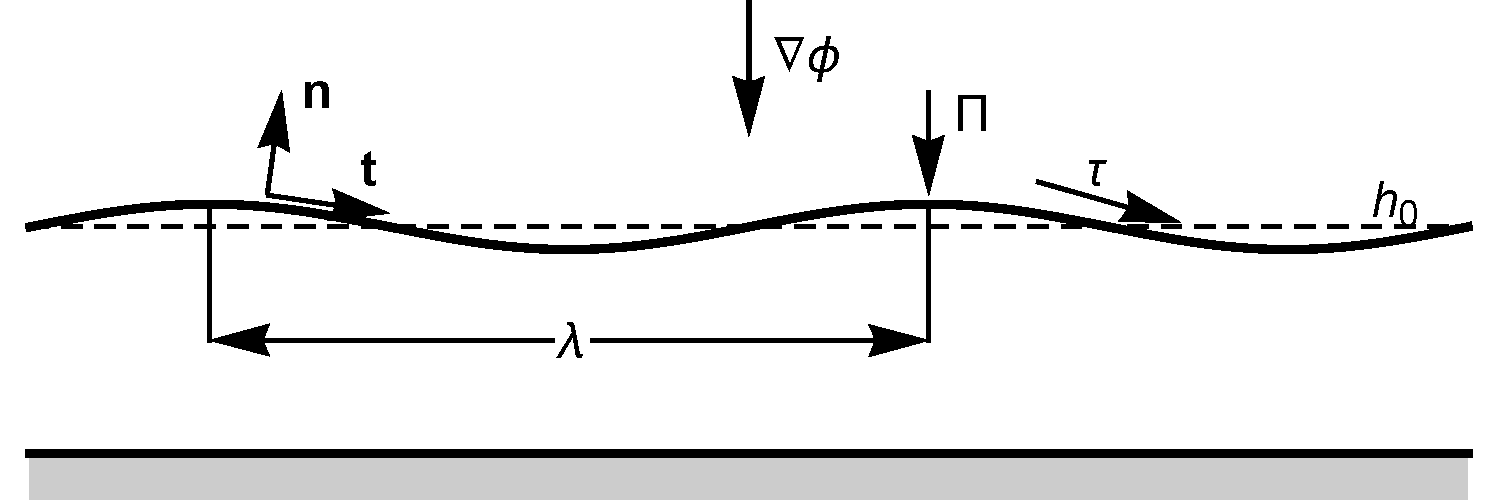
\includegraphics[scale=0.35]{Figures/ThinFilm.pdf}
      \end{center}
      \small{\begin{align*}
        U_X + W_Z &= 0 \\
        \varepsilon Re\p{U_T + U U_X + W U_Z} &= -P_X + U_{ZZ} + \varepsilon^2 U_{XX} - \Phi_X \\
        \varepsilon^3 Re\p{W_T + W W_X + W W_Z} &= -P_Z + \varepsilon^2\p{W_{ZZ} + \varepsilon^2 W_{XX}} - \Phi_Z \\
        W &= 0, U = 0 &\text{at } Z = 0 \\
        W &= H_T + U H_X &\text{at } Z = H\\
        U_Z + \varepsilon^2 W_X - 4\varepsilon^2 H_X U_X &= \tau + \Sigma_X &\text{at } Z = H \\
        -P -\Pi + \varepsilon^2U_X\p{\varepsilon^2 H_X^2 - 1} &= \varepsilon^2H_X\p{U_Z + \varepsilon^2 W_X} + C^{-1} \varepsilon^3 H_{XX} &\text{at } Z = H
      \end{align*}}
        %\v{T} \cdot \v{n} &= \p{-\kappa \sigma + \Pi}\v{n} + \p{\pd{\sigma}{s} + \tau}\v{t} &\text{at } Z = H
    \end{frame}

    \begin{frame}
      Take $\varepsilon \to 0$,
      \begin{align*}
        U_X + W_Z &= 0 \\
        U_{ZZ} &= P_X + \Phi_X \\
        0 &= -P_Z - \Phi_Z
      \end{align*}
      \begin{align*}
        W &= 0 \qquad \text{at } Z = 0 \\
        U &= 0
      \end{align*}
      \begin{align*}
        W &= H_T + U H_X  \qquad \text{at } Z = H \\
        U_Z &= \tau_0 + \Sigma_X  \\
        -\Pi_0 - P &= \bar{C}^{-1} H_{XX}
      \end{align*}
    \end{frame}

    \begin{frame}
      Integrate over $Z$ and simplify
      \begin{align*}
        0 &= H_T + \p{\dintt{0}{H}{U}{Z}}_X \\
        P + \Phi &= \eval{\Phi}{Z = H} - \bar{C}^{-1} H_{XX} - \Pi \\
        U &= \p{\tau + \Sigma_X}Z - \p{P_X + \Phi_X}\p{HZ - \frac{1}{2}Z^2} \\
        0 &= H_T + \p{\p{\tau + \Sigma_X}\frac{1}{2}H^2 - \p{P_X + \Phi_X}\frac{1}{3}H^3}_X \\
        P_X + \Phi_X &= \p{\eval{\Phi}{Z = H} - \Pi}_X - \bar{C}^{-1} H_{XXX}
      \end{align*}

      \small{\begin{gather*}
        H_T + \p{\frac{1}{2}\p{\tau + \Sigma_X}H^2 - \frac{1}{3}\p{\eval{\Phi}{Z = H} - \Pi}_X H^3}_X = - \frac{1}{3}\bar{C}^{-1}\p{H^3 H_{XXX}}_X
      \end{gather*}}
    \end{frame}

  \section{Method}
    \begin{frame}
      \frametitle{Operator Splitting}
      \begin{itemize}
        \item Simplified Model
          \[
            q_t + \p{q^2 - q^3}_x = -\p{q^3 q_{xxx}}_x \qquad \p{0, T} \times \Omega
          \]

        \item Operator Splitting
          \begin{align*}
            q_t + \p{q^2 - q^3}_x &= 0 \\
            q_t + \p{q^3 u_{xxx}}_x &= 0
          \end{align*}

        \item Strang Splitting \hfill \\
          $\frac{1}{2}\Delta t$ step of Convection
          \[
            q_t + \p{q^2 - q^3}_x = 0
          \]
          $\Delta t$ step of Diffusion
          \[
            q_t + \p{q^3 u_{xxx}}_x = 0
          \]
          $\frac{1}{2}\Delta t$ step of Convection
          \[
            q_t + \p{q^2 - q^3}_x = 0
          \]
      \end{itemize}
    \end{frame}

  \subsection{Convection}
    \begin{frame}
      \frametitle{Convection}
      \begin{itemize}
        \item Convection Equation
          \begin{gather*}
            q_t + f\p{q}_x = 0 \qquad \p{0, T} \times \Omega \\
            f(q) = q^2 - q^3
          \end{gather*}

        \item Weak Form \hfill \\
          Find $q$ such that
          \[
            \dintt*{\Omega}{}{q_t v - f(q) v_x}{x} + \eval{\hat{f}v}{\partial\Omega} = 0
          \]
          for all test functions $v$
      \end{itemize}
    \end{frame}

    \begin{frame}
      \frametitle{Notation}
      \begin{itemize}
        \item Partition the domain, $\br{a, b}$ as
          \[
            a = x_{1/2} < \cdots < x_{j-1/2} < x_{j+1/2} < \cdots < x_{N + 1/2} = b
          \]

        \item $I_j = \br{x_{j-1/2}, x_{j+1/2}}$
        \item $x_j = \frac{x_{j+1/2} + x_{j-1/2}}{2}$.
          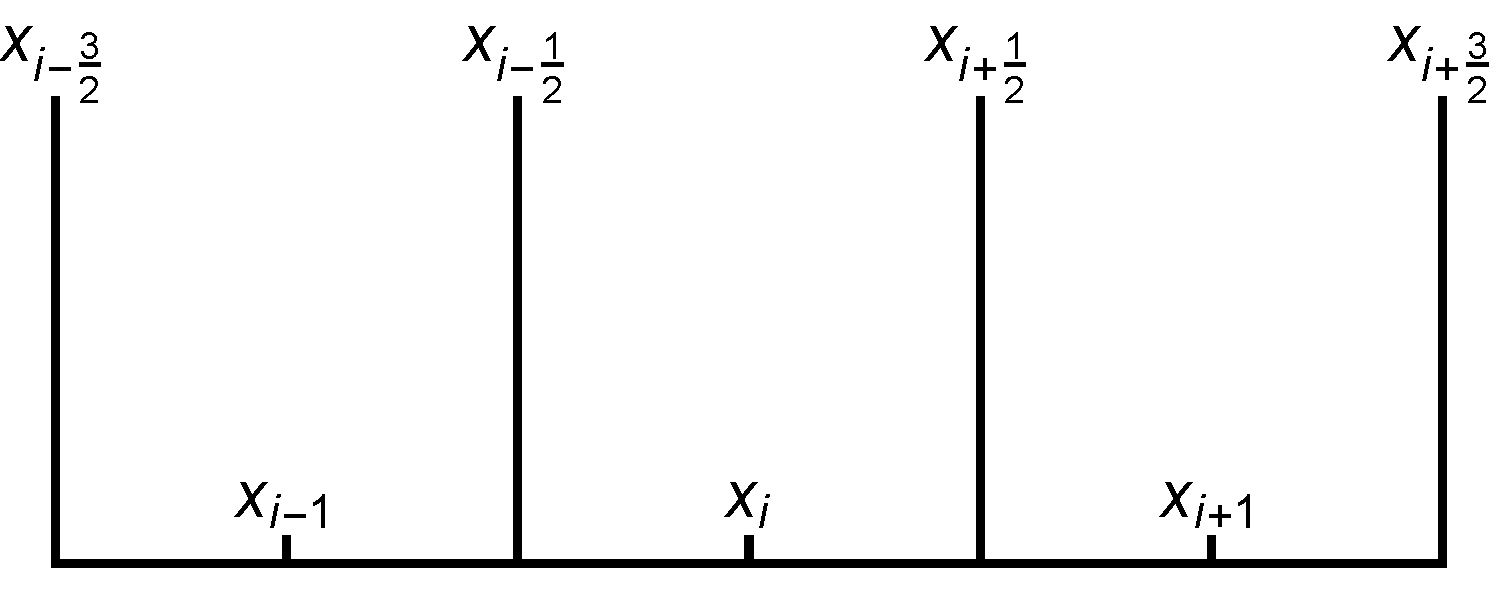
\includegraphics[scale=0.35]{Figures/Cells.pdf}
      \end{itemize}
    \end{frame}

    \begin{frame}
      \frametitle{Runge Kutta Discontinuous Galerkin}
      \begin{itemize}
        \item 
          Find $Q(t,x)$ such that for each time $t \in \p{0, T}$, $Q(t, \cdot) \in V_h = \set{v \in L^1(\Omega): \eval{v}{I_j} \in P^k(I_j)}$
          \begin{align*}
            \dintt{I_j}{}{Q_t v}{x} &= \dintt{I_j}{}{f(Q)v_x}{x} \\
            &- \p{\mcF_{j + 1/2}v^-(x_{j+1/2}) - \mcF_{j - 1/2}v^+(x_{j-1/2})}
          \end{align*}
          for all $v \in V_h$

        \item Rusanov/Local Lax-Friedrichs Numerical Flux
          \small{\[
            \mcF_{j+1/2} = \frac{1}{2}\p{f\p{Q^-_{j+1/2}} + f\p{Q^+_{j+1/2}}} + \frac{1}{2}\max[q]{\abs{f'(q)}}\p{Q^-_{j+1/2} - Q^+_{j+1/2}}
          \]}
        \vspace{-.3cm}
        \item Solve this system of ODEs with any Explicit Strong Stability Preserving (SSP) Runge-Kutta Method.
      \end{itemize}
    \end{frame}

    \begin{frame}
      \frametitle{Explicit SSP Runge Kutta Methods}
      \begin{itemize}
        \item Forward Euler
          \begin{align*}
            q^{n+1} = q^n + \Delta t L(q^n)
          \end{align*}

        \item Second Order
          \begin{align*}
            q^{\star} &= q^n + \Delta t L(q^n) \\
            q^{n+1} &= \frac{1}{2}\p{q^n + q^{\star}} + \frac{1}{2} \Delta t L(q^{\star})
          \end{align*}
      \end{itemize}
    \end{frame}

  \subsection{Diffusion}
    % \begin{frame}
      % \frametitle{Diffusion}
      % \begin{itemize}
        % \item Diffusion Equation
          % \begin{align*}
            % q_t &= -\p{q^3 q_{xxx}}_x \qquad \p{0, T} \times \Omega
          % \end{align*}

        % \item Linearize operator at $t = t^n$, let $f(x) = q^3(t = t^n, x)$
          % \[
            % q_t = -\p{f(x) q_{xxx}}_x \qquad \p{0, T} \times \Omega
          % \]
      % \end{itemize}
    % \end{frame}

    % \begin{frame}
      % \frametitle{Local Discontinuous Galerkin}
      % Find $Q(t, x), R(x), S(x), U(x)$ such that for all $t \in \p{0, T}$
      % $Q(t, \cdot), R, S, U \in V_h = \set{v \in L^1(\Omega): \eval{v}{I_j} \in P^k(I_j)}$
      % \begin{align*}
        % \dintt{I_j}{}{R v}{x} &= -\dintt{I_j}{}{Q v_x}{x} + \p{\hat{Q}_{j+1/2}v^-_{j+1/2} - \hat{Q}_{j-1/2} v^+_{j-1/2}} \\
        % \dintt{I_j}{}{S w}{x} &= -\dintt{I_j}{}{R w_x}{x} + \p{\hat{R}_{j+1/2}w^-_{j+1/2} - \hat{R}_{j-1/2} w^+_{j-1/2}} \\
        % \dintt{I_j}{}{U y}{x} &= \dintt{I_j}{}{S_x f y}{x} - \p{S^-_{j+1/2}f^-_{j+1/2}y^-_{j+1/2} - S^+_{j-1/2}f^+_{j-1/2}y^+_{j-1/2}} \\
        % &+ \p{\hat{S}_{j+1/2} \hat{f}_{j+1/2} y^-_{j+1/2} - \hat{S}_{j-1/2} \hat{f}_{j-1/2} y^+_{j-1/2}} \\
        % \dintt{I_j}{}{Q_t z}{x} &= -\dintt{I_j}{}{U z_x}{x} + \p{\hat{U}_{j+1/2}z^-_{j+1/2} - \hat{U}_{j-1/2} z^+_{j-1/2}}
      % \end{align*}
      % for all $I_j \in \Omega$ and all $v, w, y, z \in V_h$.
    % \end{frame}

    % \begin{frame}
      % \frametitle{Numerical Fluxes}
      % \begin{align*}
        % \hat{f}_{j+1/2} &= \frac{1}{2}\p{f^+_{j+1/2} + f^-_{j+1/2}} \\
        % \hat{Q}_{j+1/2} &= Q^+_{j+1/2} \\
        % \hat{R}_{j+1/2} &= R^-_{j+1/2} \\
        % \hat{S}_{j+1/2} &= S^+_{j+1/2} \\
        % \hat{U}_{j+1/2} &= U^-_{j+1/2}
      % \end{align*}
      % \begin{center}
        % 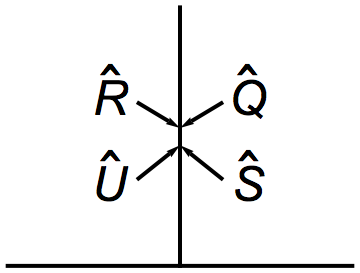
\includegraphics[scale=0.3]{Figures/localDG.png}
      % \end{center}
    % \end{frame}

    % \begin{frame}
      % \frametitle{LDG Complications}
      % \begin{itemize}
        % \item Explicit time step scales with $h^4$
        % \item Implicit System is difficult to solve efficiently
          % \begin{itemize}
            % \item GMRES iterations scale with size of system
            % \item Preconditioned GMRES
              % \begin{align*}
                % P &= A^{-1}_0 \\
                % PAx &= Pb
              % \end{align*}
            % \item Geometric Multigrid fails to converge
          % \end{itemize}
      % \end{itemize}
    % \end{frame}

    \begin{frame}
      \frametitle{Finite Difference Approach}
      \begin{itemize}
        \item Diffusion Equation
          \begin{align*}
            q_t &= -\p{q^3 q_{xxx}}_x \qquad \p{0, T} \times \Omega
          \end{align*}
        \item Let cell centers, $x_i$, form finite difference grid.
        \item Finite difference space, $\RR^N$.
        \item $Q_{DG} \in V_h \to Q_{FD} \in \RR^N$
          \[
            \p{Q_{FD}}_i = \frac{1}{h}\dintt{K_i}{}{Q_{DG}}{x}
          \]

        \item $Q_{FD} \in \RR^N \to Q_{DG} \in V_h$
          \begin{align*}
            \eval{Q_{DG}}{K} &\in P^1(K) \\
            \frac{1}{h}\dintt{K_i}{}{Q_{DG}}{x} &= \p{Q_{FD}}_i \\
            \eval{\partial_x Q_{DG}}{K_i} &= \frac{\p{Q_{FD}}_{i+1} - \p{Q_{FD}}_{i-1}}{2h}
          \end{align*}
      \end{itemize}
    \end{frame}

    \begin{frame}
      \frametitle{Finite Difference Approximation}
      \begin{itemize}
        \item First derivative approximation
          \[
            \p{-\p{f(x) q_{xxx}}_x}_i \approx -\frac{f_{i+1/2}\p{q_{xxx}}_{i+1/2} - f_{i-1/2}\p{q_{xxx}}_{i-1/2}}{h}
          \]

        \item Third derivative approximation
          \[
            \p{q_{xxx}}_{i+1/2} \approx \frac{-Q_{i-1} + 3Q_i - 3Q_{i+1} + Q_{i+2}}{h^3}
          \]

        \item Value of $Q^3$ at boundary
          \[
            f_{i+1/2} = q^3_{i+1/2} = \p{\frac{Q_i + Q_{i+1}}{2}}^3
          \]

        \item Full operator
          \[
            L(q) = L(f = q^3, q) = A(f)q
          \]
      \end{itemize}
    \end{frame}

    \begin{frame}
      \frametitle{Implicit L-Stable Runge Kutta}
      \begin{itemize}
        \item Backward Euler
          \begin{align*}
            q^{n+1} = q^n + \Delta t L(q^{n+1})
          \end{align*}

        \item 2nd Order
          \begin{align*}
            q^{\star} &= q^n + \frac{1}{4} \Delta t \p{L(q^n) + L(q^{\star})} \\
            3 q^{n+1} &= 4 q^{\star} - q^{n} + \Delta t L(q^{n+1})
          \end{align*}
      \end{itemize}
    \end{frame}

    \begin{frame}
      \frametitle{Nonlinear Solvers}
      \begin{itemize}
        \item Picard Iteration
          \begin{align*}
            % L(q) &= A(f \approx q^3) q \\
            q^{n+1}_0 &= q^n
          \end{align*}
          \begin{align*}
            q^{n+1}_{m+1} &= q^n + \Delta t L\p{f = \p{q^{n+1}_m}^3, q^{n+1}_{m+1}}
          \end{align*}
          \begin{align*}
            q^{\star}_{m+1} &= q^n + \frac{1}{4} \Delta t \p{L(q^n) + L\p{f = \p{q^{\star}_m}^3, q^{\star}_{m+1}}} \\
            3 q^{n+1}_{m+1} &= 4 q^{\star} - q^{n} + \Delta t L\p{f = \p{q^{n+1}_m}^3, q^{n+1}_{m+1}}
          \end{align*}
        % \item Newton's Method
          % \begin{align*}
            % q^{n+1}_{m+1} = q^{n+1}_m - J{(q^{n+1}_m)}^{-1}F(q^{n+1}_m)
          % \end{align*}
          % \begin{align*}
            % F(q) &= q - q^n - \Delta t L(q) \\
            % J(q) &= I - \Delta t L'(q)
          % \end{align*}
          %\begin{align*}
            %F(q) &= q - q^n - \frac{1}{4} \Delta t \p{L(q^n) + L(q)} \\
            %J(q) &= I - \frac{1}{4}\Delta t L'(q) \\
            %F(q) &= 3 q - 4 q^{\star} + q^{n} - \Delta t L(q) \\
            %J(q) &= 3I - \Delta t L'(q)
          %\end{align*}
      \end{itemize}
    \end{frame}

  \section{Numerical Results}
    \begin{frame}
      \frametitle{Manufactured Solution}
      \begin{align*}
        q_t + \p{q^2 - q^3}_x &= -\p{q^3 q_{xxx}}_x + s(x,t) \\
        q_t + \p{q^2 - q^3}_x &= s(x, t) \\
        q_t &= -\p{q^3 q_{xxx}}_x \\
        q(x, t) &= 0.1*\sin{2\pi(x - t)} + 0.15
      \end{align*}
      \begin{center}
      \begin{tabular}{rllll}
        \toprule
        \multicolumn{5}{c}{1st Order} \\
        \midrule
            & \multicolumn{2}{c}{1 Iteration} & \multicolumn{2}{c}{2 Iterations} \\
        \midrule
        $N$      & error   & order & error  & order \\
        \midrule
        25       & 0.1529  & ---   & 0.0776 & ---  \\
        50       & 0.05334 & 1.52  & 0.0370 & 1.06 \\
        100      & 0.02374 & 1.16  & 0.0177 & 1.06 \\
        200      & 0.01186 & 1.00  & 0.0091 & 0.95 \\
        \bottomrule
      \end{tabular}
      \end{center}
    \end{frame}

    \begin{frame}
      \frametitle{Manufactured Solution}
      \begin{align*}
        q_t + \p{q^2 - q^3}_x &= -\p{q^3 q_{xxx}}_x + s(x,t) \\
        q_t + \p{q^2 - q^3}_x &= s(x, t) \\
        q_t &= -\p{q^3 q_{xxx}}_x \\
        q(x, t) &= 0.1*\sin{2\pi(x - t)} + 0.15
      \end{align*}
      \begin{center}
      \begin{tabular}{rllllll}
        \toprule
        \multicolumn{7}{c}{2nd Order} \\
        \midrule
            & \multicolumn{2}{c}{1 Iteration} & \multicolumn{2}{c}{2 Iterations} & \multicolumn{2}{c}{3 Iterations} \\
        \midrule
        $N$ & error & order & error & order & error & order\\
        \midrule
        25  & 0.03449 & ---  & 0.02890 & ---  & 0.03103 & --- \\
        50  & 0.01061 & 1.70 & 0.00875 & 1.72 & 0.00910 & 1.77 \\
        100 & 0.00330 & 1.68 & 0.00197 & 2.14 & 0.00202 & 2.17 \\
        200 & 0.00143 & 1.20 & 0.00051 & 1.96 & 0.00051 & 1.98 \\
        \bottomrule
      \end{tabular}
      \end{center}
    \end{frame}

    \begin{frame}
      \frametitle{Manufactured Solution}
      \begin{align*}
        q_t + \p{q^2 - q^3}_x &= -\p{q^3 q_{xxx}}_x + s(x,t) \\
        q_t + \p{q^2 - q^3}_x &= s(x, t) \\
        q_t &= -\p{q^3 q_{xxx}}_x \\
        q(x, t) &= \frac{2}{10} e^{-10\p{x - t - \frac{3}{2}}^2} + \frac{1}{10}
      \end{align*}
      \begin{center}
      \begin{tabular}{rllll}
        \toprule
        \multicolumn{5}{c}{2nd Order} \\
        \midrule
            & \multicolumn{2}{c}{1 Iteration} & \multicolumn{2}{c}{2 Iterations} \\
        \midrule
        $N$ & error & order & error & order\\
        \midrule
        50  & 0.05609 & ---  & 0.3808 & ---  \\
        100 & 0.04178 & 0.42 & 0.2335 & 0.7  \\
        200 & 0.01182 & 1.82 & 0.0429 & 2.44 \\
        400 & 0.00612 & 0.94 & 0.0104 & 2.04 \\
        800 & 0.00268 & 1.19 & 0.0026 & 2.03 \\
        \bottomrule
      \end{tabular}
      \end{center}
    \end{frame}

    % \begin{frame}
      % \frametitle{Manufactured Solution with Newton's Method}
      % \begin{align*}
        % q_t &= -\p{q^3 q_{xxx}}_x + s(x,t) \\
        % q(x, t) &= \frac{2}{10} e^{-10t} e^{-300\p{x - \frac{1}{2}}^2} + \frac{1}{10}
      % \end{align*}
      % \begin{center}
      % \begin{tabular}{rll}
        % \toprule
        % \multicolumn{3}{c}{Backward Euler} \\
        % \midrule
        % $N$ & error & order \\
        % \midrule
         % 50 & 0.0280 & --- \\
        % 100 & 0.0153 & 0.8765 \\
        % 200 & 0.0080 & 0.9249 \\
        % 400 & 5.5e75 & -258 \\
        % \bottomrule
      % \end{tabular}
      % \end{center}
    % \end{frame}

  \subsection{Travelling Waves}
    \begin{frame}
      \frametitle{Hyperbolic Wave Structure}
      \begin{itemize}
        \item Conservation Law
          \[
            q_t + f{(q)}_x = 0
          \]
        \item Riemann Problem Initial Data
          \[
            q(x, 0) =
            \begin{cases}
              q_l & x < d \\
              q_r & x > d
            \end{cases}
          \]

        \item Rankine-Hugoniot Condition
          \[
            s = \frac{f(q_l) - f(q_r)}{q_l - q_r}
          \]
      \end{itemize}
    \end{frame}

    \begin{frame}
      \frametitle{Convex Flux Function}
      \begin{itemize}
        \item Shock Wave
          \[
            f'(q_l) > s > f'(q_r)
          \]
          \begin{center}
            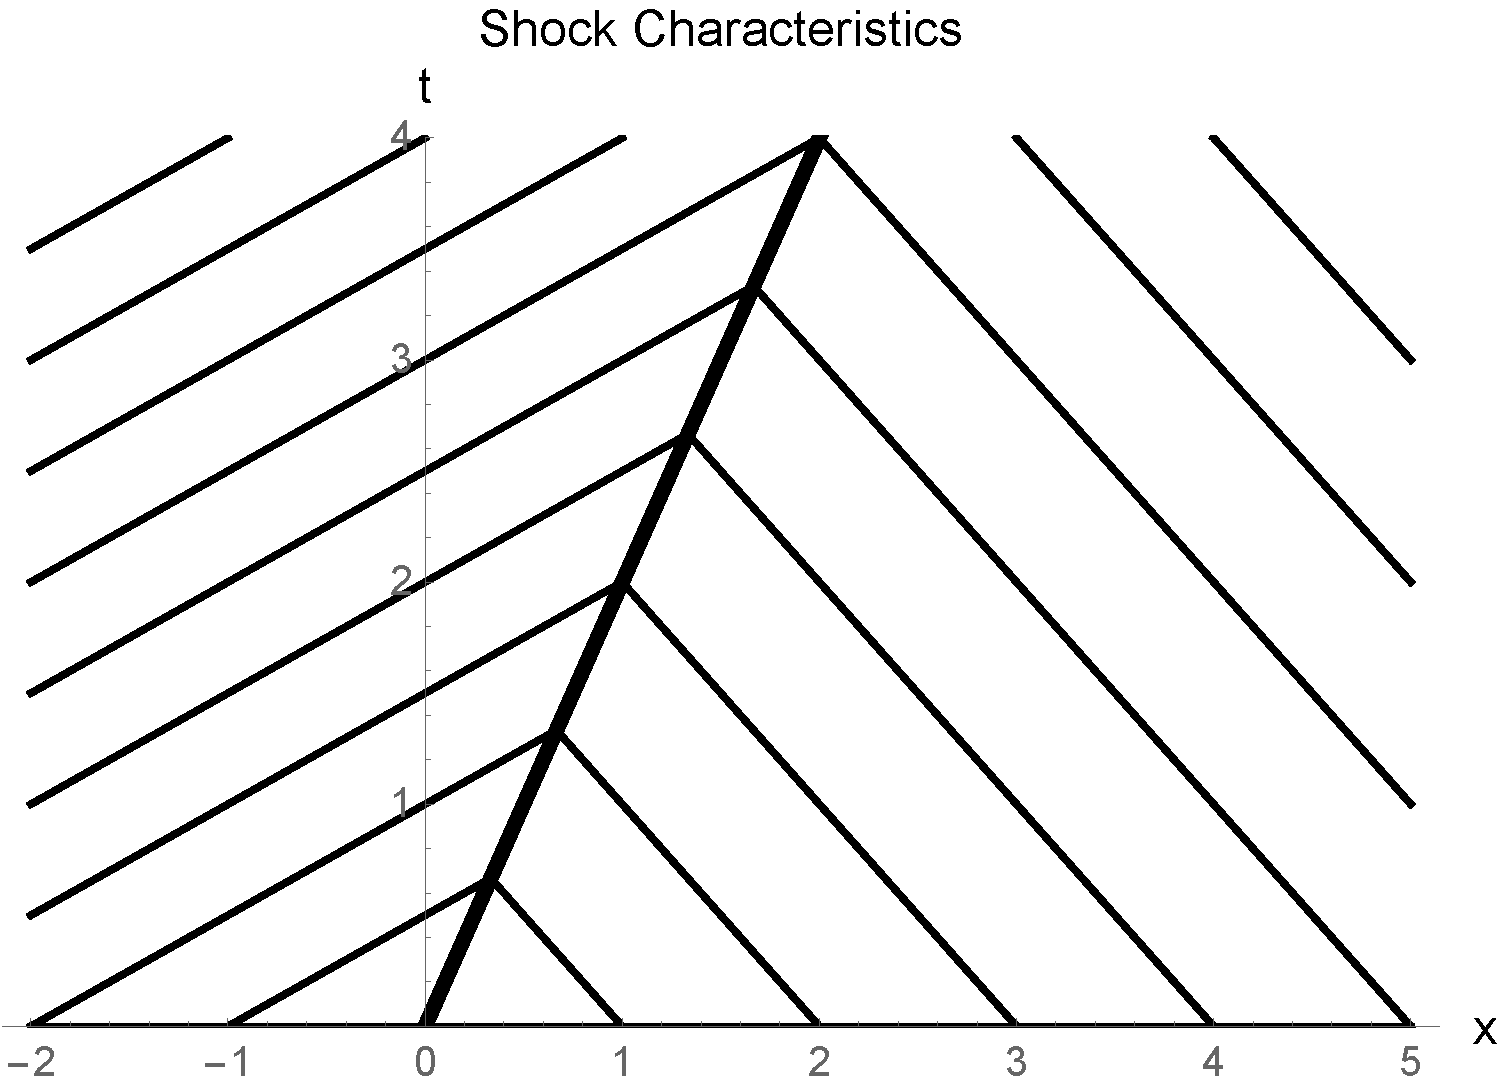
\includegraphics[scale=0.13]{Figures/ShockCharacteristics.pdf}
            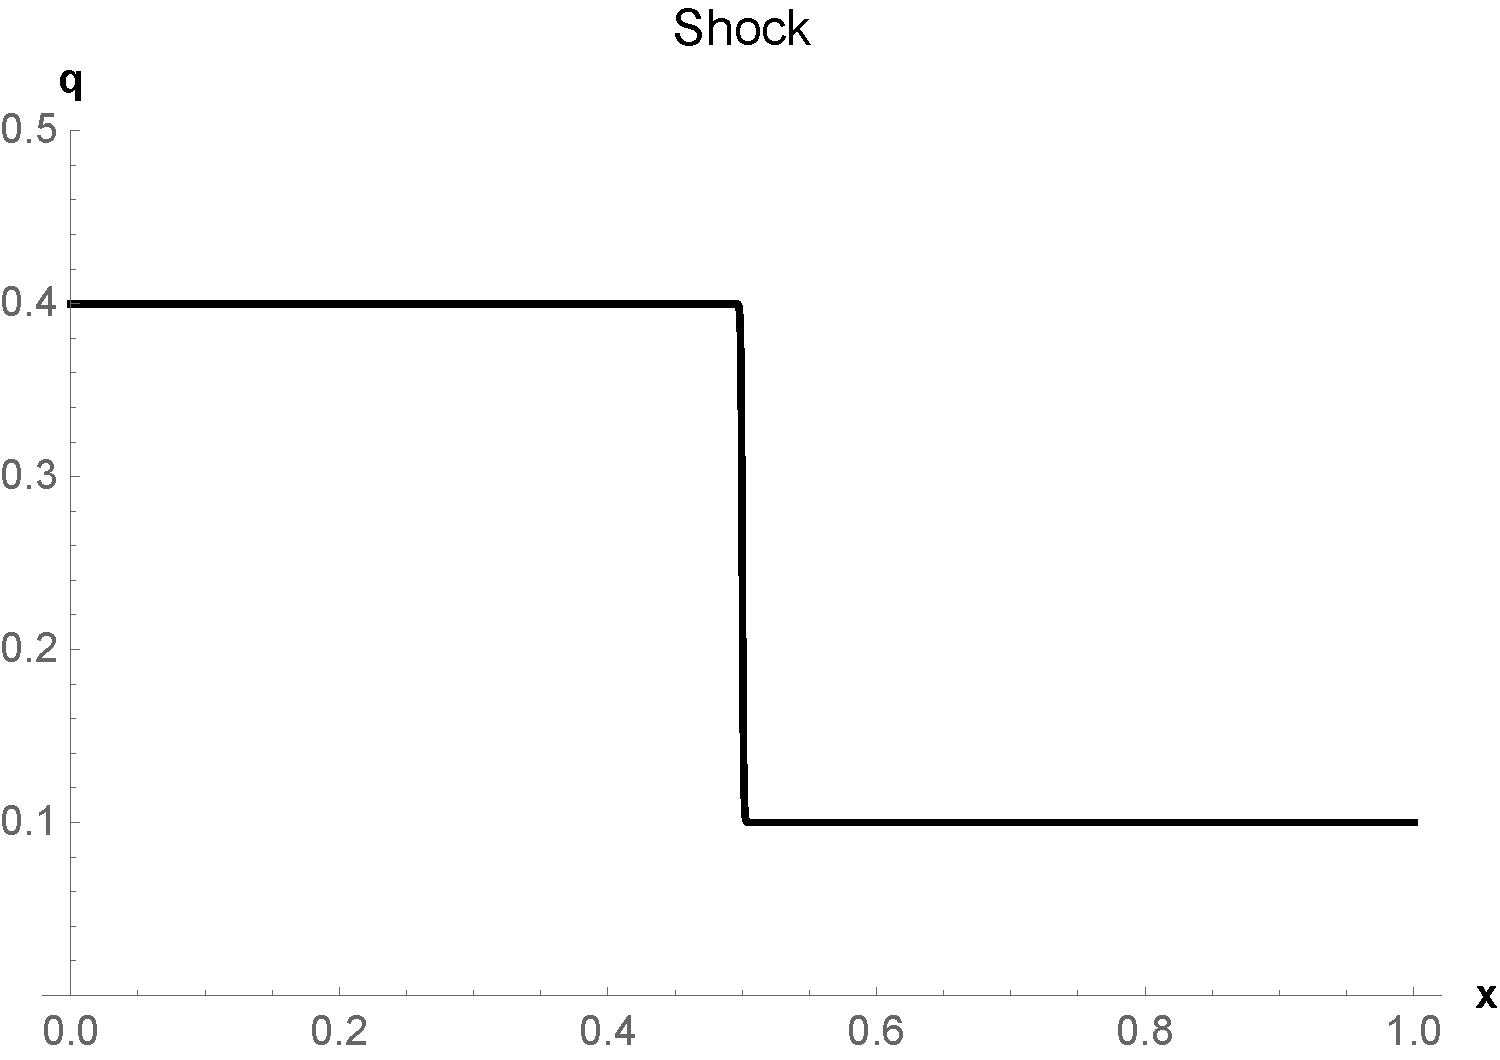
\includegraphics[scale=0.13]{Figures/CompressiveShock.pdf}
          \end{center}
        \item Rarefaction
          \[
            f'(q_l) < s < f'(q_r)
          \]
          \begin{center}
            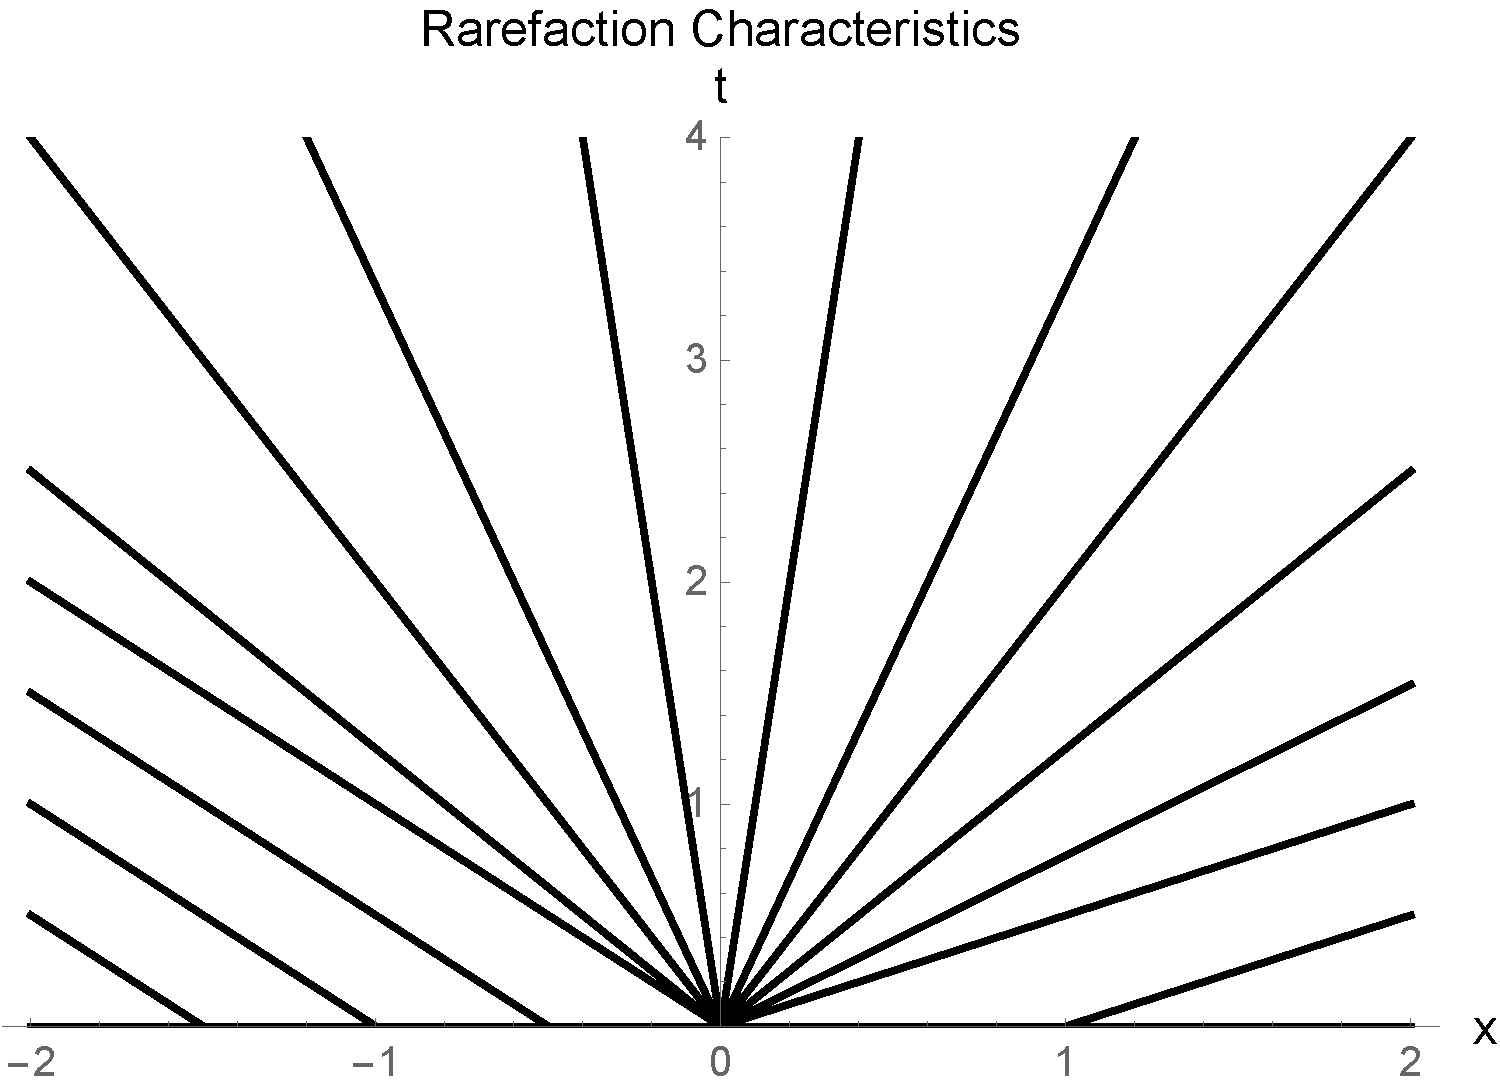
\includegraphics[scale=0.13]{Figures/RarefactionCharacteristics.pdf}
            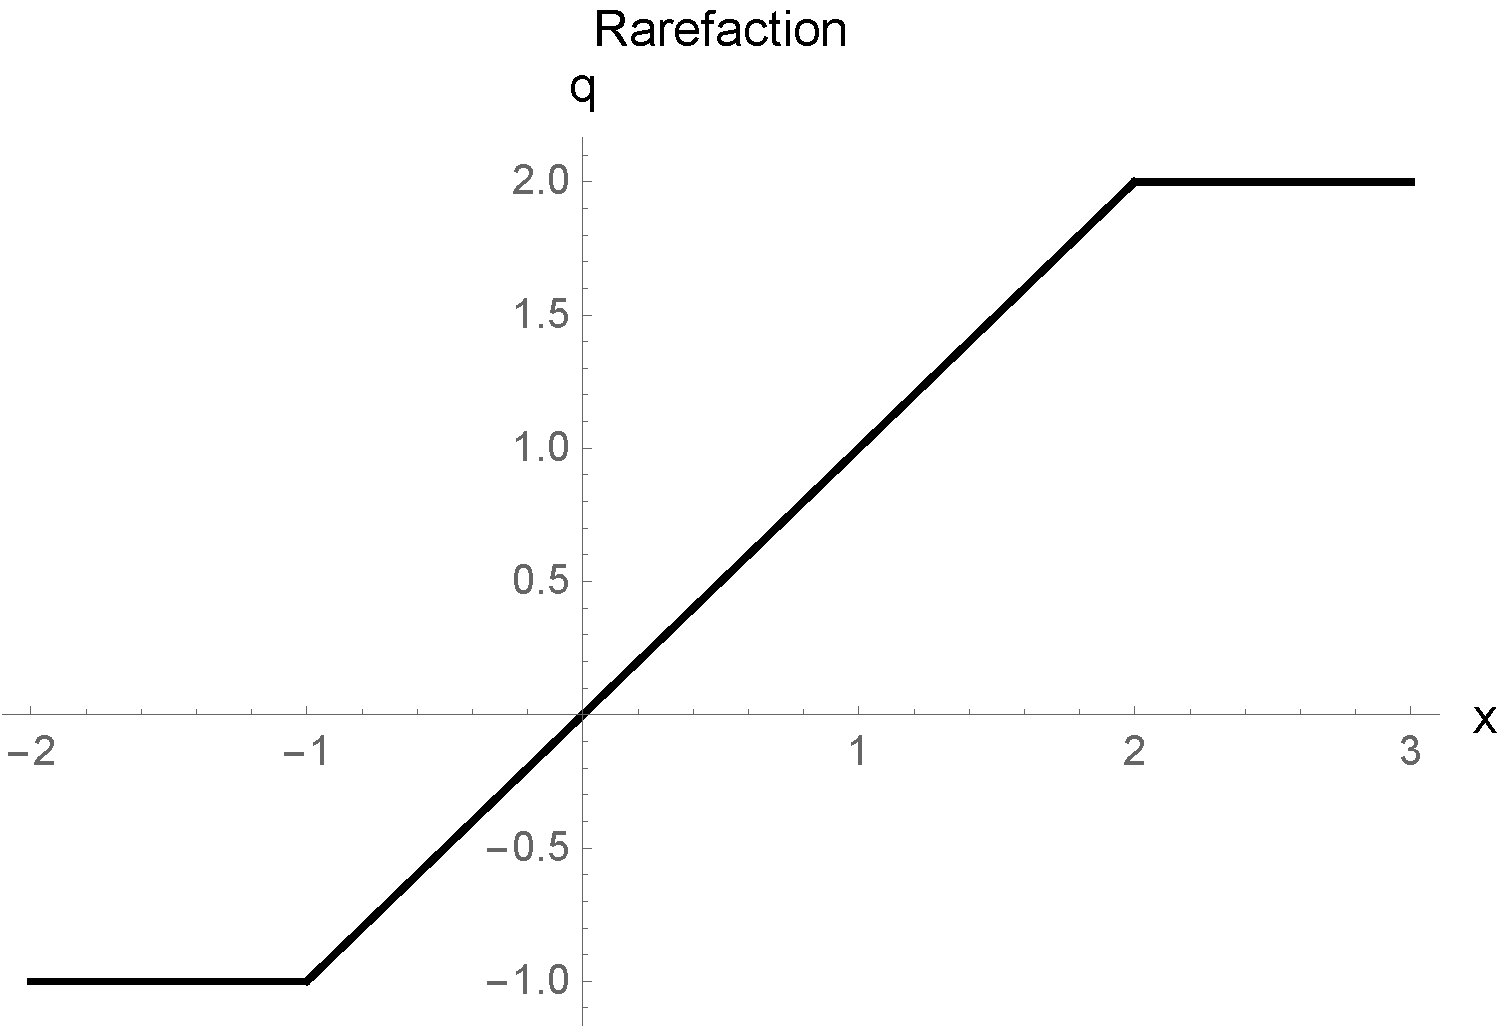
\includegraphics[scale=0.13]{Figures/Rarefaction.pdf}
          \end{center}
      \end{itemize}
    \end{frame}

    \begin{frame}
      \frametitle{Nonconvex Flux Function}
      \[
          q_t + \p{q^2 - q^3}_x = 0
      \]
      \begin{center}
        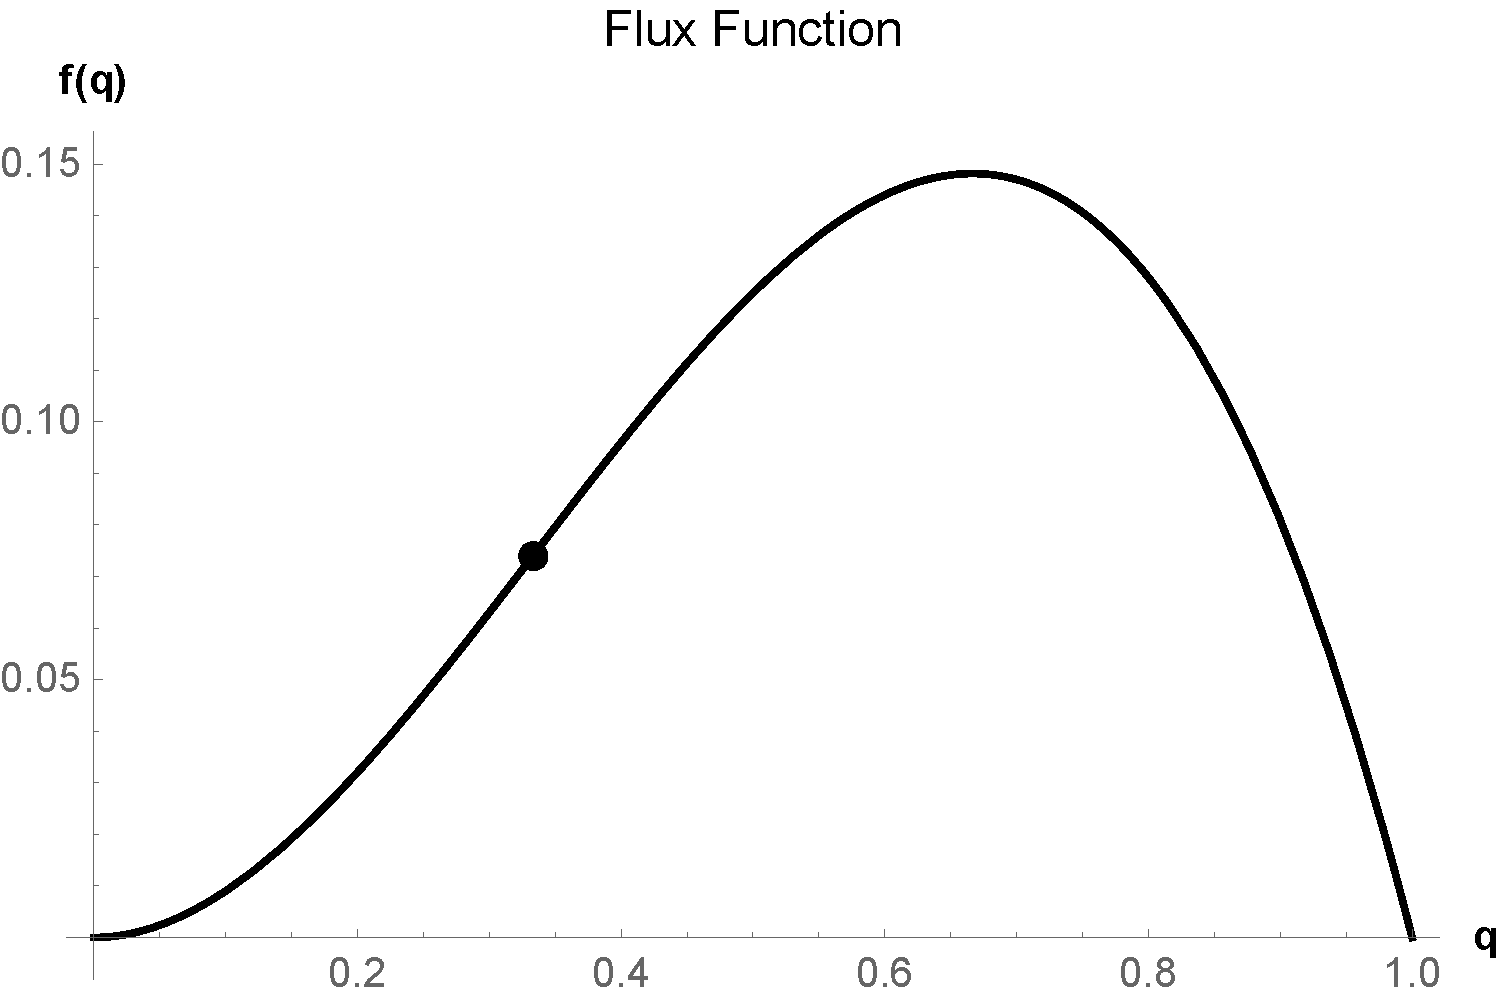
\includegraphics[scale=0.35]{Figures/FluxFunctionNonconvex.pdf}
      \end{center}
    \end{frame}

    \begin{frame}
      \frametitle{Nonconvex Flux Function}
      \begin{align*}
        f'(q_b) &= s \\
        q_b &= (1 - q_r)/2 
      \end{align*}
      \begin{center}
        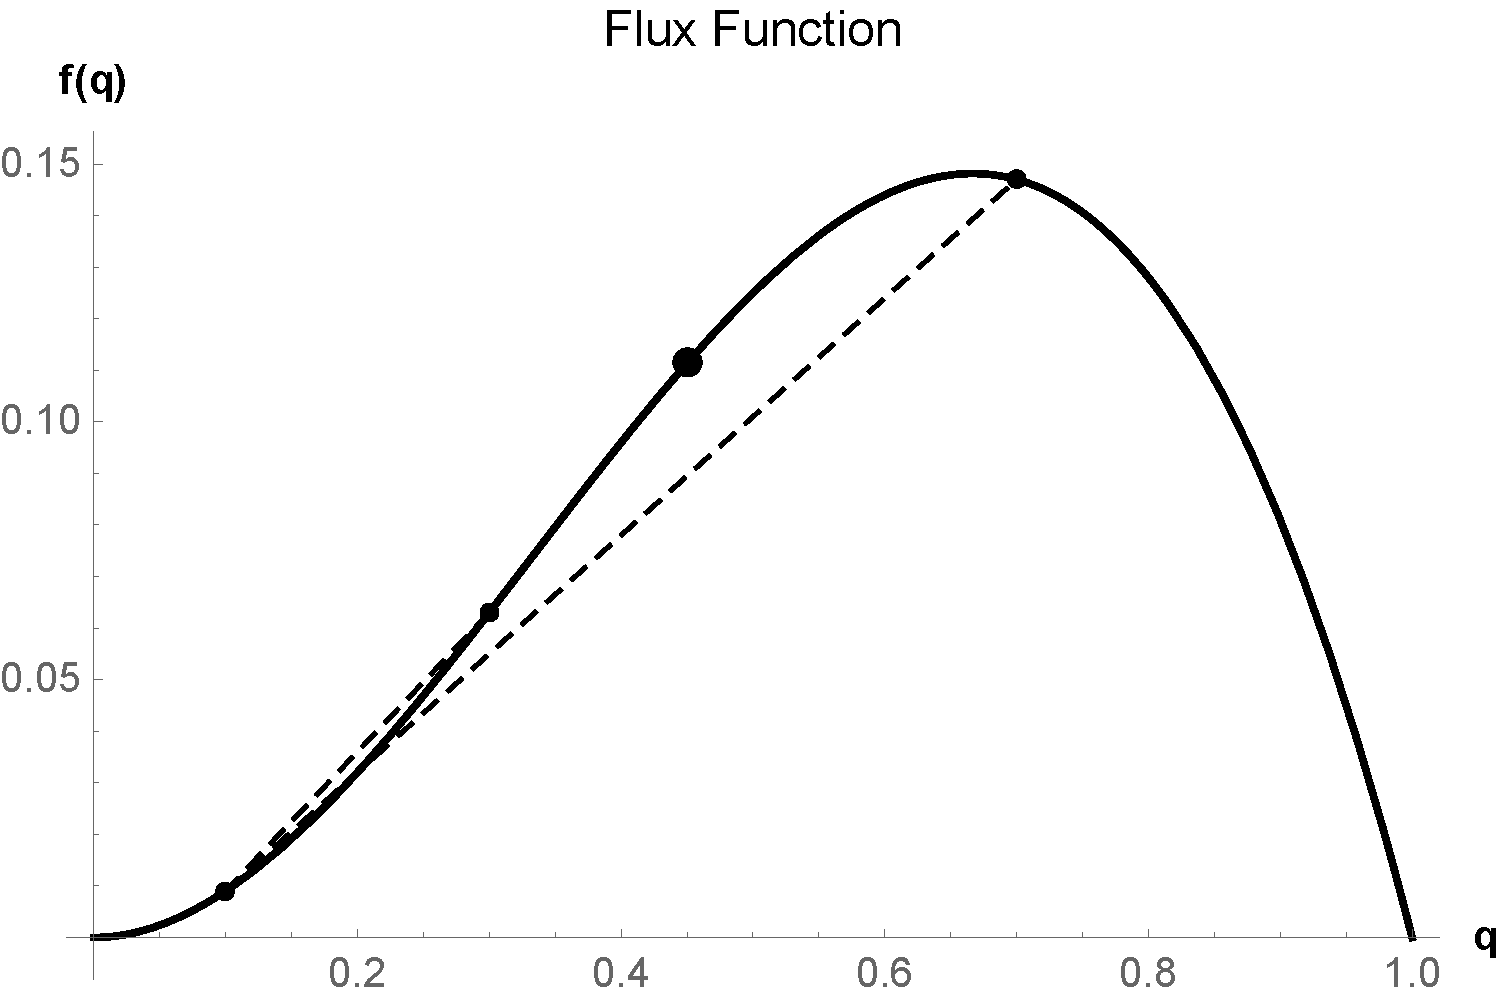
\includegraphics[scale=0.35]{Figures/FluxFunction2Cases.pdf}
      \end{center}
    \end{frame}

    \begin{frame}
      \frametitle{Compressive Shock}
      \begin{align*}
        q_l &< q_b \\
        q(x, t) &=
        \begin{cases}
          q_l & x \le st \\
          q_r & x > st
        \end{cases}
      \end{align*}
      \begin{center}
        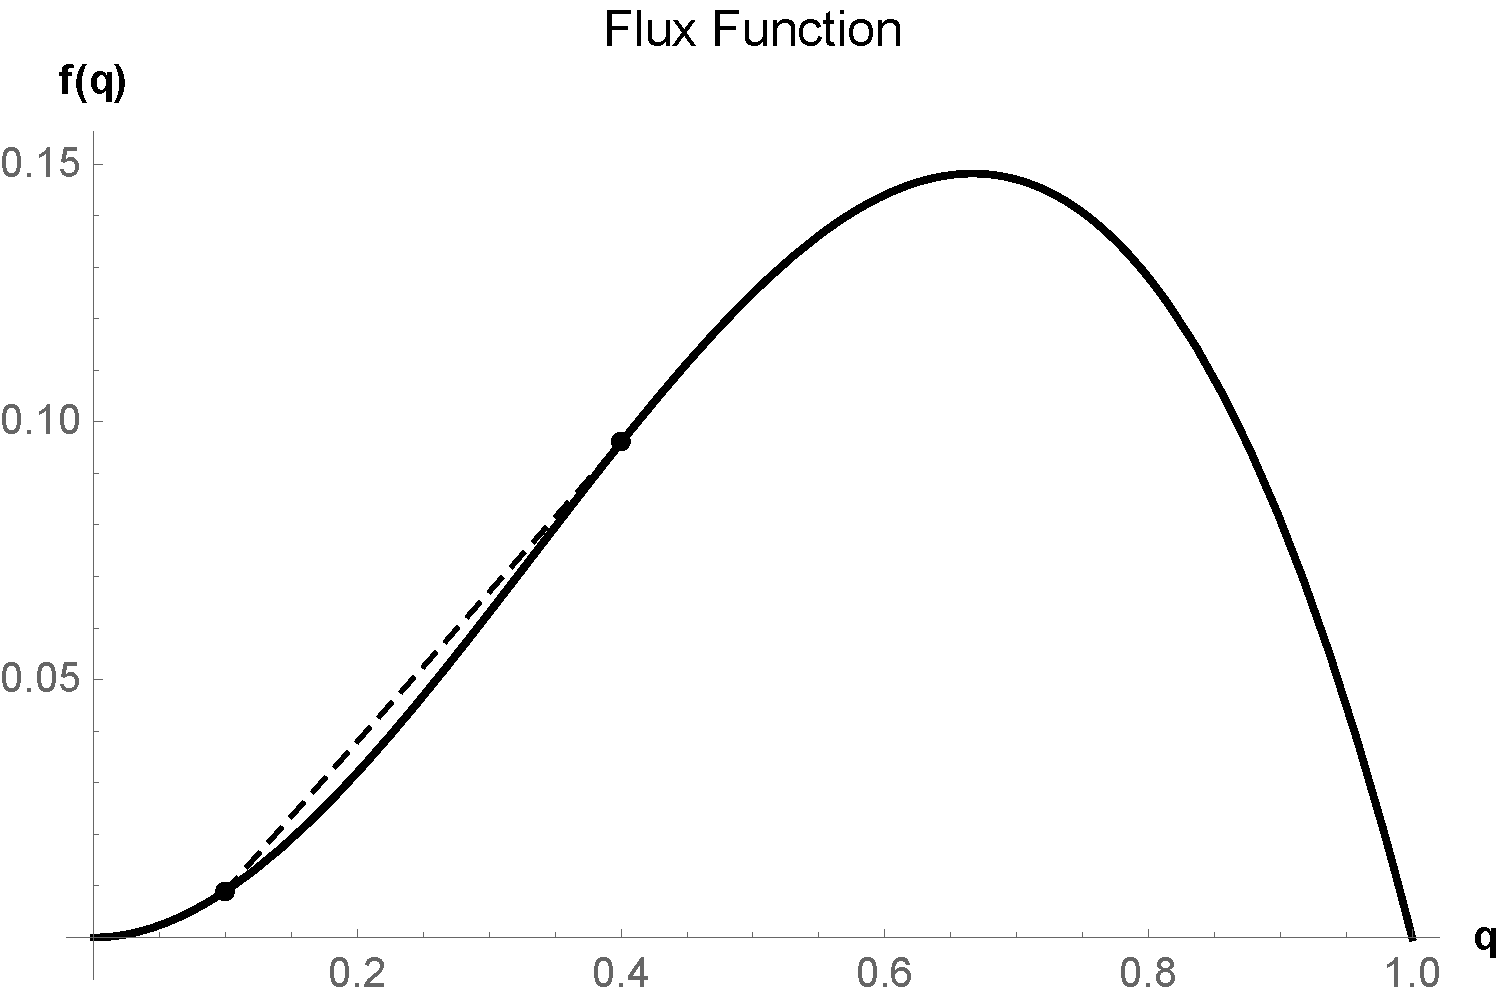
\includegraphics[scale=0.2]{Figures/FluxFunctionCompressiveShock.pdf}
        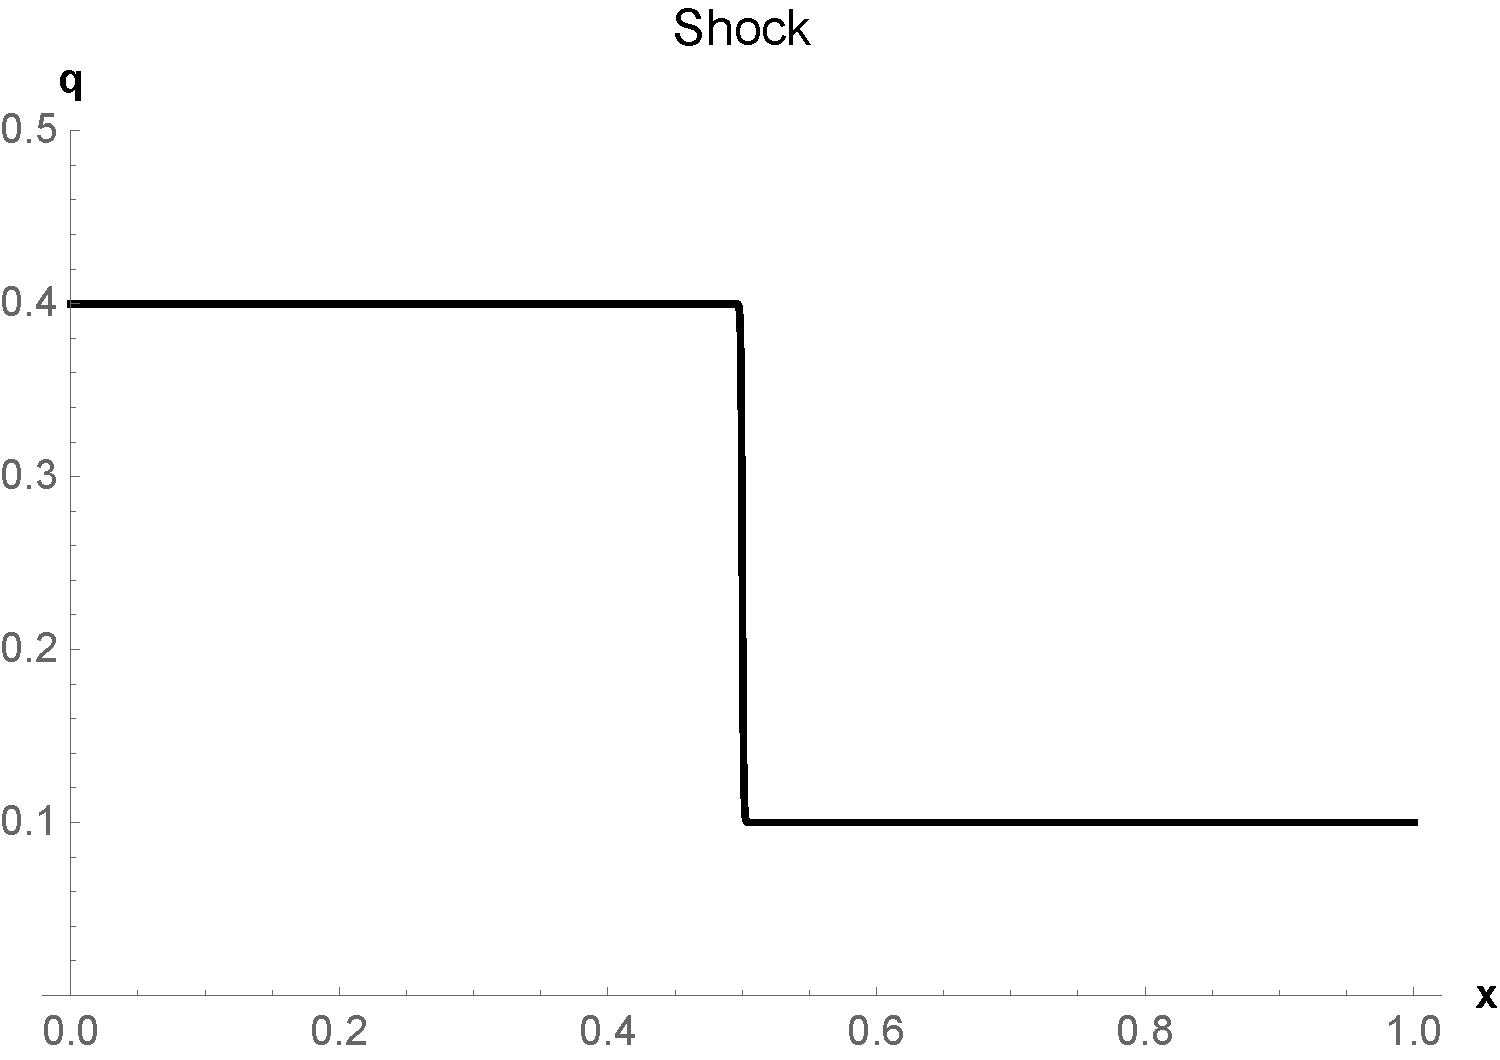
\includegraphics[scale=0.2]{Figures/CompressiveShock.pdf}
      \end{center}
    \end{frame}

    \begin{frame}
      \frametitle{Rarefaction-Compressive Shock}
      \begin{gather*}
        q_l > q_b \\
        q(x, t) =
        \begin{cases}
          q_l & x < f'(q_l)t \\
          h_r(x) & f'(q_l)t < x < f'(q_b)t \\
          q_r & x > f'(q_b)t
        \end{cases}
      \end{gather*}
      \begin{center}
        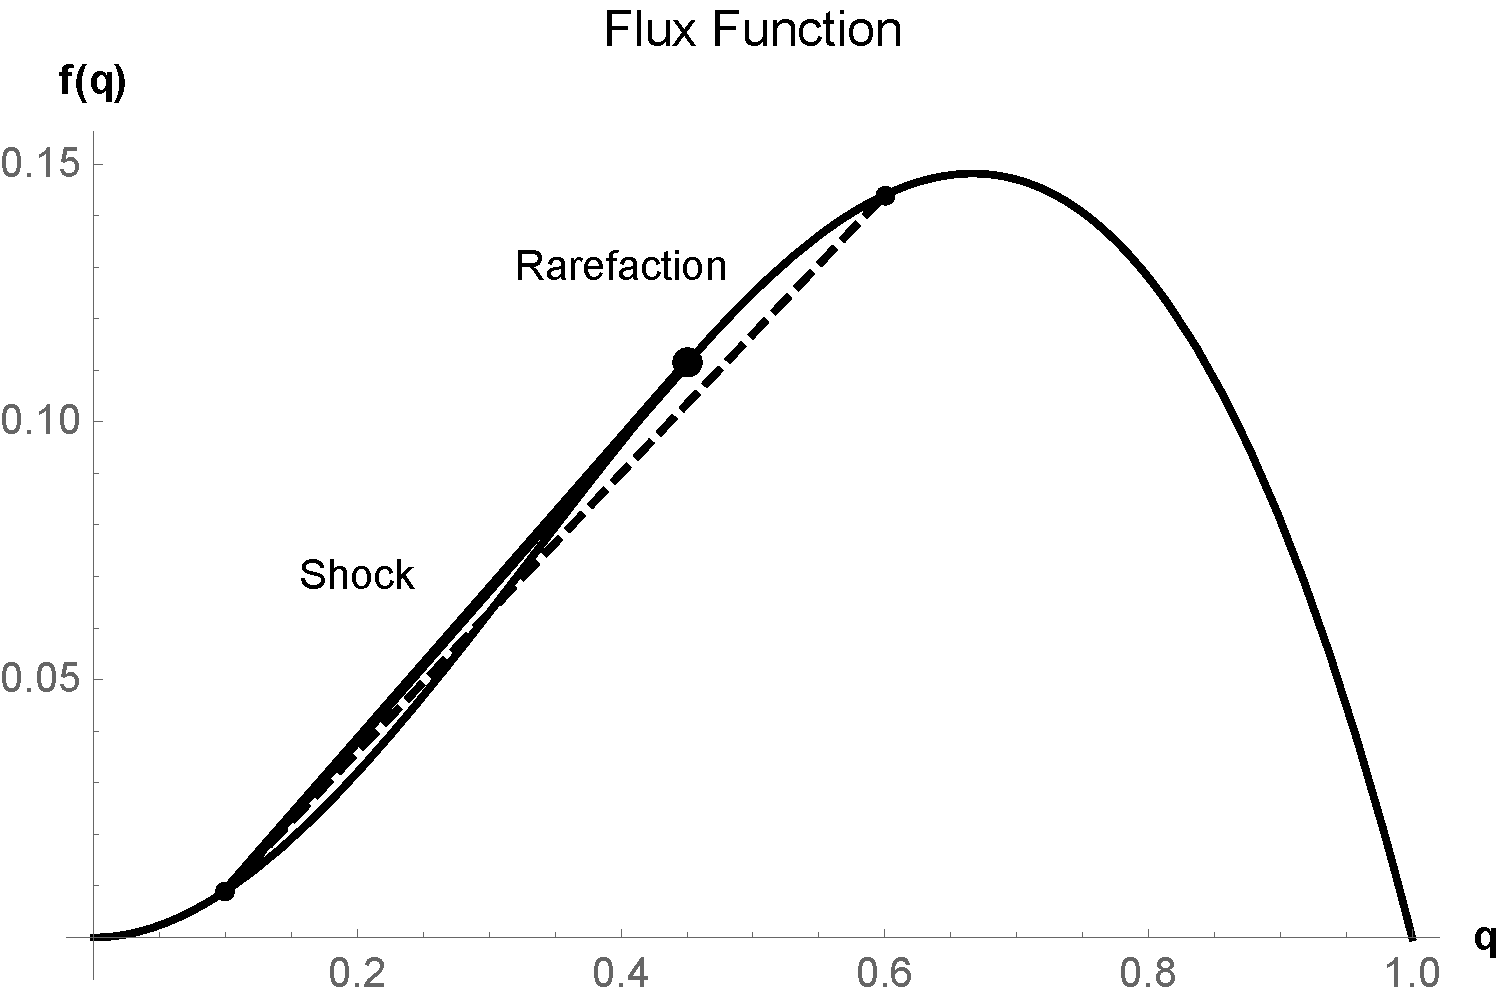
\includegraphics[scale=0.2]{Figures/FluxFunctionRarefactionShock.pdf}
        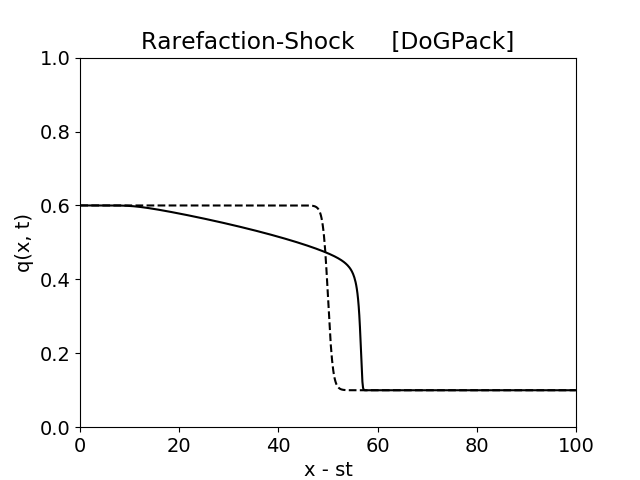
\includegraphics[scale=0.3]{Figures/RarefactionShock.png}
      \end{center}
    \end{frame}

    \begin{frame}
      \frametitle{Wave Structure with Nonlinear Hyper Diffusion}
      \[
        q_t + \p{q^2 - q^3}_x = -\p{q^3q_{xxx}}_x
      \]
      \[
        q_r = 0.1 \qquad q_l = 0.3
      \]
      \begin{center}
        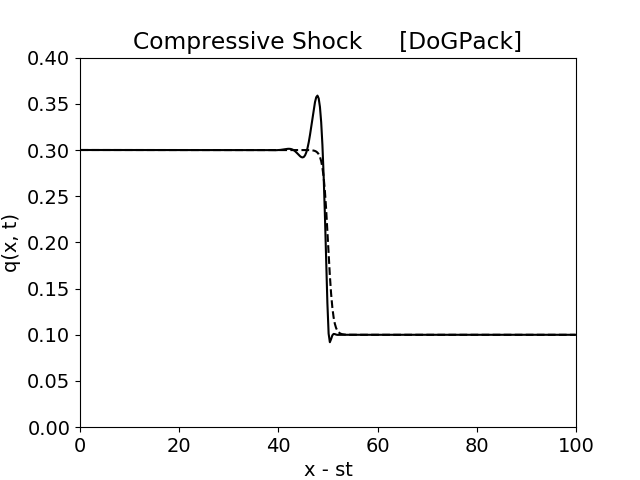
\includegraphics[scale=0.4]{Figures/case1.png}
      \end{center}
    \end{frame}

    \begin{frame}
      \frametitle{Wave Structure with Nonlinear Hyper Diffusion}
      \[
        q_r = 0.1 \qquad q_l = 0.3323
      \]
      \[
        q(x, 0) = \p{-\tanh{x - 50} + 1}\frac{q_l - q_r}{2} + q_r
      \]
      \begin{center}
        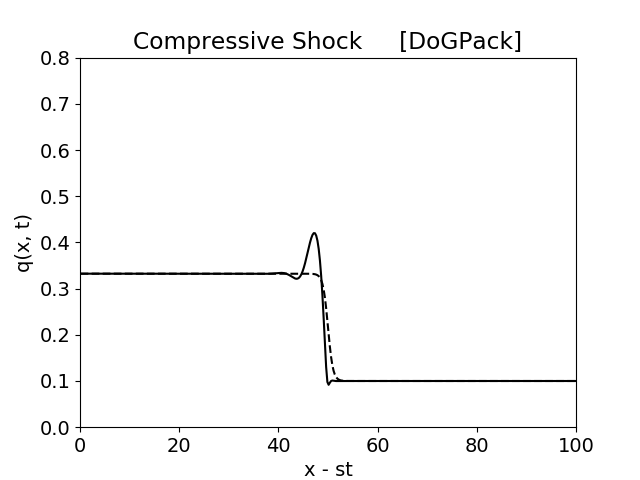
\includegraphics[scale=0.4]{Figures/case2_1.png}
      \end{center}
    \end{frame}

    \begin{frame}
      \frametitle{Wave Structure with Nonlinear Hyper Diffusion}
      \[
        q_r = 0.1 \qquad q_l = 0.3323 \qquad q_m = 0.6
      \]
      \[
        q(x, 0) = 
        \begin{cases}
          \frac{q_m - q_l}{2}\tanh{x - 50} + \frac{q_m + q_l}{2} & x < 55 \\
          -\frac{q_m - q_r}{2}\tanh{x - 60} + \frac{q_m + q_r}{2} + q_r & x > 55 \\
        \end{cases}
      \]
      \begin{center}
        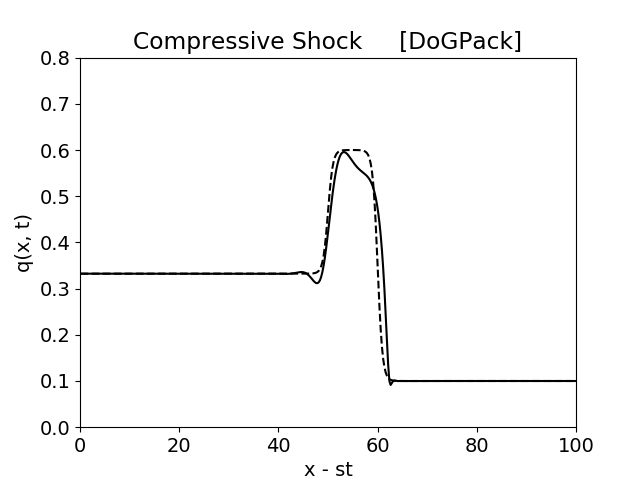
\includegraphics[scale=0.4]{Figures/case2_2.png}
      \end{center}
    \end{frame}

    \begin{frame}
      \frametitle{Wave Structure with Nonlinear Hyper Diffusion}
      \[
        q_r = 0.1 \qquad q_l = 0.4
      \]
      \[
        q(x, 0) = \p{-\tanh{x - 300} + 1}\frac{q_l - q_r}{2} + q_r
      \]
      \begin{center}
        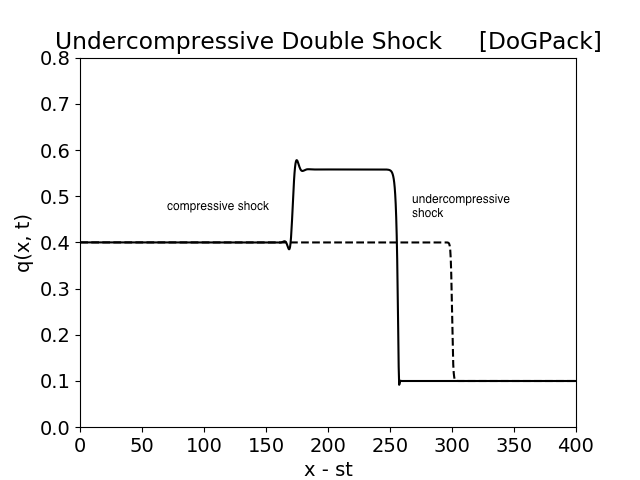
\includegraphics[scale=0.4]{Figures/case3.png}
      \end{center}
    \end{frame}

    \begin{frame}
      \frametitle{Wave Structure with Nonlinear Hyper Diffusion}
      \[
        q_r = 0.1 \qquad q_l = 0.8
      \]
      \[
        q(x, 0) = \p{-\tanh{x - 1100} + 1}\frac{q_l - q_r}{2} + q_r
      \]
      \begin{center}
        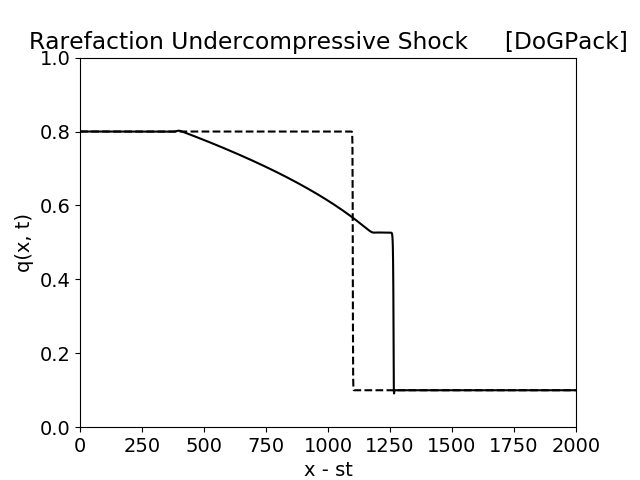
\includegraphics[scale=0.4]{Figures/case4.png}
      \end{center}
    \end{frame}

  \section{Conclusion}
    \begin{frame}
      \frametitle{Conclusion}
      Observations
      \begin{itemize}
        \item Nonlinear Hyper Diffusion has subtle instabilities
      \end{itemize}
      Future Work
      \begin{itemize}
        \item Higher Order Convergence
          \begin{itemize}
            \item Runge Kutta IMEX
            \item Local Discontinuous Galerkin Method
            \item Hybridized Discontinuous Galerkin Method
          \end{itemize}
      \end{itemize}
    \end{frame}

    \begin{frame}
      Questions?
    \end{frame}

    \begin{frame}[allowframebreaks]
      \frametitle{Bibliography}
      % TODO: Bibliography
      \nocite{*}
      \printbibliography{}
    \end{frame}
\end{document}
